\documentclass[a4paper, 12pt]{article}

\usepackage{czech}
\usepackage{graphicx}
\usepackage[utf8]{inputenc}
\usepackage{listings}
\usepackage{url}
% \usepackage{a4wide}

\def\CS{$\cal C\kern-.1667em\lower.5ex\hbox{$\cal S$}\kern-.075em $}
\DeclareUrlCommand\url{\def\UrlLeft{<}\def\UrlRight{>} \urlstyle{tt}}

\lstset{language=Java}

\begin{document}
\begin{titlepage}

\includegraphics[bb=0 0 167 96]{fav_cmyk.pdf}
\vfill
\begin{center}
{\huge Umělá inteligence a rozpoznávání}\\[3ex]
{\Large Expertní genealogický systém}
\end{center}
\vfill
\begin{tabbing}
Vypracoval: \hspace{1ex}\=Zdeněk Janeček\kill
Vypracoval: \>Zdeněk \textsc{Janeček}\\[1ex]
Datum:\> \today
\end{tabbing}
\end{titlepage}

\section{Zadání}
Vytvořte genealogický expertní systém. Vstupem bude informace databáze
základních informací o osobě [id, jméno, matka, otec, pohlaví, partner].
Program bude umět odpovídat na otázky: Kdo je můj pokrevní příbuzný?
Kolik má moje prateta sestřenic? Jaký je vtah mezi Petrem a Pavlem?\ldots
a další podobné.

\section{Analýza}
% grafové prohledávání, datové struktury
Rodinný strom je z hlediska grafové teorie n-ární strom, protože mám dva
rodiče a neomezeně mnoho dětí. Pokud zanedbám manželství a postavím
strom jen ze vztahů rodič--potomek, bude acykličnost zachována.
Manželství není dokonce stálé a stačí si ho tedy pouze zaznamenat.
Společné děti manželů, také nejsou jisté, tudíž je praktičtější ukládat
si potomky u každého rodiče zvlášť.

Abych mohl ukládat rodinný strom je třeba stanovit kořen. Máme tedy
dvě varianty. Kořenem bude jeden společný potomek, a nebo společná
matka. Obě varianty jsou rovnocené, protože ve výsledku v programu
procházím strom nezávisle na kořenovém uzlu. Zvolil jsem jako superuzel
matku, která dostala id 0.

Pro ukládání dat o rodině jsem vytvořil jednoduchý formát souboru.
Na obrázku \ref{fig:family} vidíte následující položky:

\begin{enumerate}
\setcounter{enumi}{-1}
\item ID
\item Jméno
\item (červeně) id natky
\item (žluté) id otce
\item (zelené) true -- muž, false -- žena
\item (modře) partner
\end{enumerate}

Když víme počet položek z prvního řádku, algoritmus je pak jednoduchý:
\begin{enumerate}
\item načti atributy
\item když neexistuje odkazovaná osoba, vytvoř základ
\item přidej se jako dítě rodiče a nastav partnera
\item pokud ještě neexistuji, vytvoř se
\item opakuj krok 1 pro další osobu
\end{enumerate}

\begin{figure}
\centering
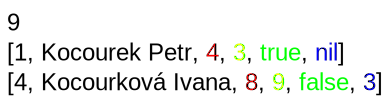
\includegraphics{format_family}
\caption{Formát souboru s rodinnými daty.}
\label{fig:family}
\end{figure}

\section{Design}
% Expertní a klientská třída, UI
Aplikace bude konsolová. Při psaní do terminálu se hodí escape sekvence,
které umožňují mazat konkrétní kusy obrazovky a tím dosáhnout určité
interaktivity. Budou stačit pouhé dva způsoby vstupu a to id osoby a
požadovaný vztah. V hlavičce programu se bude vypisovat formulovaná
otázka.

Uvnitř programu zastupuje třída \texttt{NTree} rodinný strom. Tato třída je
konstruována s parametrem souboru s rodinnými daty. Při vytvoření
se soubor načte a uloží pole všech instancí třídy \texttt{Node}.
Každý \texttt{Node} představuje jednu osobu. Procházení
stromu je pak rychlé, protože, můžu využít jak tabulku tak
odkaz na sousední uzel.

Další část je práce s expertními daty. Bylo třeba navrhnout jak
reprezentovat rodinný vztah. Využil jsem predikátové logiky,
která je dostatečně univerzální pro práci s množinou prvků.
Definoval jsem například:

\begin{displaymath}
P(x,a) \wedge P(a,b) \wedge C(b,c) \wedge N(c,a) \rightarrow \mbox{\emph{c} je sourozenec rodičů}
\end{displaymath}

Vystačil jsem si se třemi funkcemi říkající:
\begin{description}
\item[P(a,b)] rodiče termu \emph{a} jsou \emph{b}.
\item[C(a,b)] děti termu \emph{a} jsou \emph{b}.
\item[N(a,b)] term \emph{a} neobsahuje prvky z \emph{b}.
\end{description}

Soubor jsem navrhl podobně. Stačilo se zbavit závorek a konjunkcí,
které budou platit vždy a není tedy nutné je ukládat. Soubor má formát
podle obrázku \ref{fig:expert}. První řádek je opět počet položek
v tomto souboru. Každé pravidlo má dva řádky. První z nich obsahuje
popis vztahu a na dalším je samotné pravidlo.

\begin{figure}
\centering
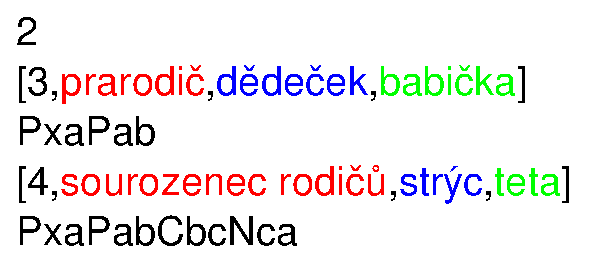
\includegraphics{format_expert}
\caption{Formát souboru s expertními daty.}
\label{fig:expert}
\end{figure}

\section{Shrnutí}
Při psaní jsem několikrát lehce změnil návrh. V počátku jsem o expertním
systému nevěděl vůbec nic. Ve výsledku jsem použil již ověřené postupy.

\end{document}
